\subsection{Player Interfaces}
\noindent First responders are equipped with a `mobile responder tool' providing sensing and awareness capabilities in three tabs (geiger cou\-nter, map, messaging and tasks; see Figure \ref{fig:ui}). The first tab shows a reading of radioactivity, player health level (based on exposure), and a GPS-enabled map of the game area to locate fellow responders, the targets to be rescued and the drop off zones for the targets. The second tab provides a broadcast messaging interface to communicate with fellow first responders and the commander $H$. The third tab shows the team and task allocation dynamically provided by the agent $PA$ that can be accepted or rejected. Notifications are used to alert both to new messages and task allocations.

\begin{figure}[htbp]
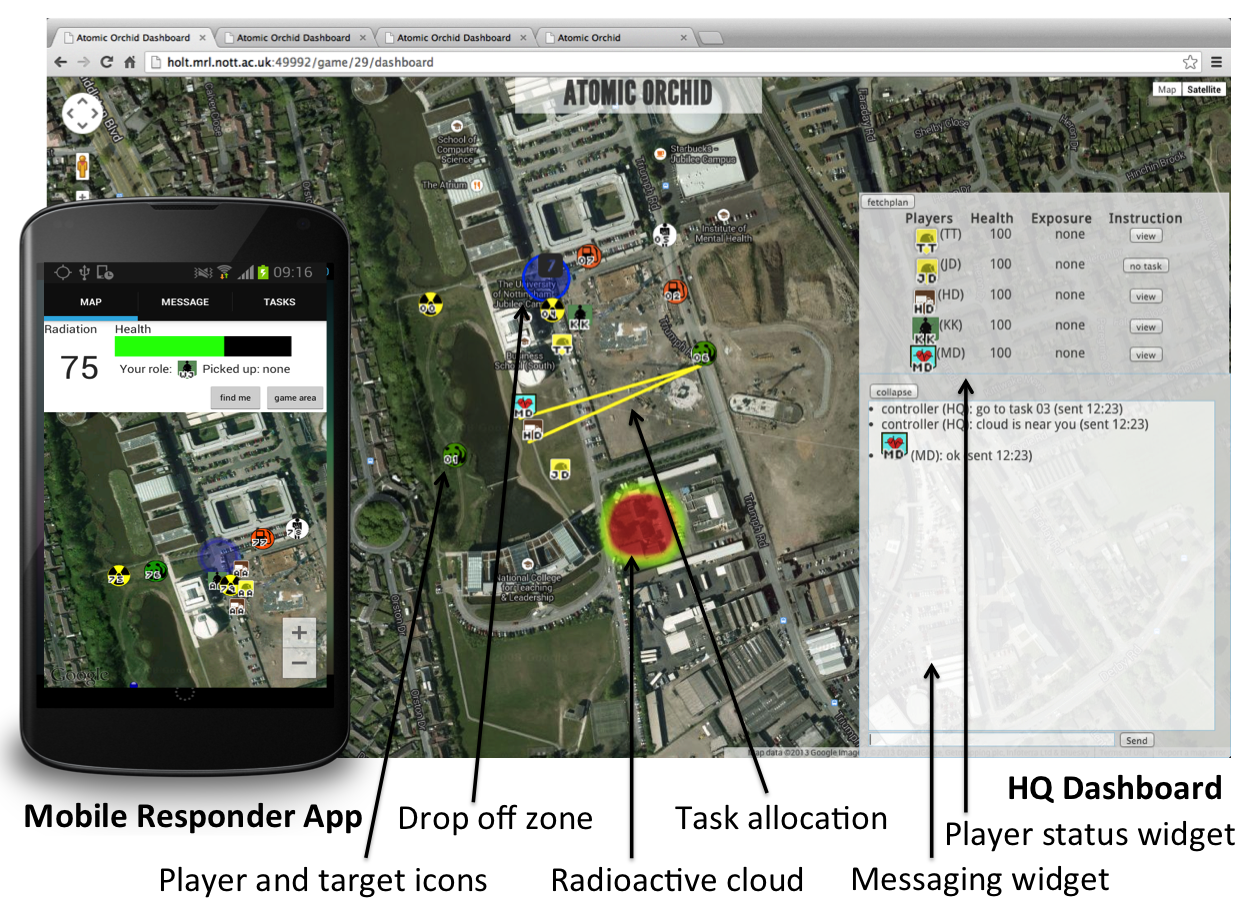
\includegraphics[width=\columnwidth]{UI.png}
\caption{Mobile first responder and HQ interfaces.}\vspace{-3mm}
\label{fig:ui}
\end{figure}

$H$ has at her disposal an `HQ dashboard' that provides an over\-view of the game area, including real-time information of the players' locations (see Figure \ref{fig:ui}). The dashboard provides a broadcast messaging widget, and a player status widget so that the responders' exposure and health levels can be monitored. $H$ can further monitor the  current team and task allocations to individual responders by $PA$ (by clicking on a button). The radioactive cloud is graphically depicted as a heatmap (`Hotter'  (red) zones correspond to higher levels of radiation). Crucially, only  $H$ can 'see' the entire cloud, while field responders are restricted to seeing a reading for their current location on their Geiger counters --- this is a deliberate design choice to require frequent communication between HQ and field responders. 

\subsection{System Architecture}
\noindent AtomicOrchid is based on the open-sourced geo-fencing game MapAttack\footnote{\url{http://mapattack.org}.} that has been iteratively developed for a responsive, (relatively) scalable experience.  The location-based game is underpinned by client-server architecture, that relies on real-time data streaming between client and server. Client-side requests for less dynamic content use HTTP. Frequent events (e.g., location updates and radiation exposure) are streamed to clients to avoid the overhead of HTTP. In this way, first responders are kept informed in near real-time. Finally,  to build the mobile app, we adapted the existing MapAttack Android app.

%The platform is built using the geoloqi platform, Sinatra for Ruby, and state-of-the-art web technologies such as socket.io, node.js and the Google Maps API. 

\subsection{Integrating the Planning Agent}
\noindent The planning agent $PA$ takes the game status (i.e., positions of players, known status of the cloud, and messages received from players) as input and produces a plan for each responder  for the current state. $PA$ is deployed on a separate server. The AtomicOrchid server requests a plan from the agent via a stateless HTTP interface by transmitting the game status in JSON format. Polling (and thus re-planning) is triggered by two types of game events:
\begin{itemize}
\item \textit{Completion of task}. On successful rescue of a target, a new plan (i.e., allocation of tasks to each responder) is requested from the agent.
\item \textit{Explicit reject}. On rejection of a task allocation by any of the allocated first responders, a new plan is requested.  More importantly, the rejected allocation is, in turn, used as a constraint within the optimisation run by the planner agent (as described in Section \ref{sec:adaptive}). For example, if two responders, one medic and one soldier, were allocated a task and the medic rejected it, the planning agent would rerun the optimisation algorithm with the constraint that this medic should not be allocated this task. If another medic is free (and accepts) the soldier and this medic can go ahead and complete the task. Otherwise, a new plan is created for the soldier.
\end{itemize} 

\todo{GOPAL: add architecture diagram showing how agent and human interact}

%\subsection{Interacting with planning agent}
%There can interact directly with field players through a task tab (Figure xx) and agent plans are also visible to HQ's dashboard interface.
Once a plan is received from $PA$, the AtomicOrchid game engine splits the plan for a given team into individual task allocations for each player and sends them to their mobile responder app. The app presents the task allocation in the task tab, detailing: i) the responder to team up with, ii) the allocated target (using target id), and iii) approximate direction of the target (e.g., north, east).  Once a player accepts a task, an acknowledgement is sent to their teammate, while rejecting a task triggers a new assignment from $PA$. 

%Furthermore, $H$ is provided with a visualisation of task allocations for each player on demand (by button press), to help monitor the task allocation computed by the agent.

